\documentclass[11pt]{article}
\usepackage[margin=1in]{geometry}
\usepackage[T1]{fontenc}
\usepackage{graphicx}
\usepackage[numbers]{natbib}
\usepackage{hyperref}
\setlength{\parskip}{0.5em}
\setlength{\parindent}{0pt}

\title{What are the newest approaches to continual learning and avoiding catastrophic forgetting?}
\author{GraphIV --- deep research}
\date{\today}

\begin{document}
\maketitle

\begin{abstract}
(round-1 saturation overridden — one more look) The review is a complete and highly detailed synthesis of the provided literature, covering the entire temporal range from origins to the 2026 frontier with no missing papers.
\end{abstract}

\section{Navigating the Stability-Plasticity Dilemma: A Comprehensive Survey of Continual Learning}

The ability of artificial intelligence to acquire knowledge incrementally is essential for transitioning from static, task-specific models to autonomous, lifelong learners. However, this transition is fundamentally obstructed by catastrophic forgetting, a phenomenon where the acquisition of new information leads to the abrupt erasure of previously learned representations. This instability creates a critical tension between plasticity, the capacity to integrate new knowledge, and stability, the preservation of existing skills. As machine learning systems move toward real-world deployment in dynamic, non-stationary environments, developing robust mechanisms to mitigate this interference has become one of the most vital challenges in modern neural architecture design.

This review traces the historical and technical evolution of the field, beginning with the foundational approaches of replay and regularization designed to stabilize weight updates during sequential training. We then examine the shift toward structural adaptation and parameter isolation to protect specific neural components, alongside meta-learning and Bayesian frameworks that attempt to manage plasticity through probabilistic modeling. The discussion expands into advanced replay and generative memory mechanisms, as well as gradient-based optimization and projection methods that refine how models navigate the loss landscape to prevent interference. Finally, we explore the current frontier of the field, focusing on the rise of transformer-based and prompt-based continual learning, and conclude by investigating emerging paradigms such as zero-forgetting and knowledge transfer.

\subsection{Foundations of Continual Learning: Replay and Regularization}

Continual learning aims to mitigate catastrophic forgetting—the dramatic performance degradation in old tasks when learning new ones [\citep{2302.00487}]. The literature establishes two primary paradigms for addressing this: replay-based methods and regularization-based methods [\citep{2007.00487}]. Replay processes generally fall into two categories: rehearsal, which involves saving a core-set of past samples [\citep{2007.00487}], and generative replay, which utilizes generative models to reconstruct past experiences [\citep{2007.00487}].

Replay methods can be implemented without task identity or explicit task boundaries, a significant advantage for real-world deployment. For instance, CLEAR utilizes an actor-critic framework, employing the Importance Weighted Actor-Learner Architecture (IMPALA) and the V-Trace off-policy algorithm to mix new and replayed experiences [\citep{1811.11682}]. This approach is noted for its ability to reduce forgetting more effectively than prior methods and its potential for combination with other strategies [\citep{1811.11682}].

In contrast, regularization-based approaches attempt to preserve knowledge by constraining parameter updates or utilizing generative models to regularize the learning process. One significant advancement in generative regularization is the use of energy-based models (EBM) with Langevin dynamic sampling [\citep{1912.01238}]. This method overcomes the deficiency of the parameter independence assumption found in variational continual learning by using a contrastive loss and Langevin dynamics as an implicit regularization term, demonstrating empirical success on Permuted-MNIST, Split-MNIST, and Fashion-MNIST [\citep{1912.01238}]. Similarly, latent variable models using variational inference (akin to VAEs) have been proposed to relax the constraints of having no access to past data or no storage of task-specific models [\citep{1810.10612}].

While many complex regularization and parameter-isolation methods have been proposed, recent analysis suggests that simpler data-driven regularization can be superior. Learning Without Forgetting (LwF) utilizes knowledge distillation loss between the previous and current models, leveraging a feature extractor and task-specific classifier heads to preserve previous task outputs using only current task data [\citep{2107.12304}]. Critically, LwF has been shown to be more effective for task-incremental learning than many more complex regularization-based and parameter-isolation methods [\citep{2107.12304}].

The tension between these approaches often lies in the trade-off between the storage requirements of rehearsal and the complexity of generative modeling. While generative methods like EBMs [\citep{1912.01238}] or latent variable models [\citep{1810.10612}] avoid storing raw data, they require sophisticated training to ensure the generated distributions accurately represent past tasks. Conversely, replay methods like CLEAR [\citep{1811.11682}] provide robust performance in reinforcement learning settings but must manage the efficiency of the replayed experience mixture. Ultimately, the field continues to evolve through taxonomies that categorize these methods by weight regularization—such as adding quadratic penalties based on parameter importance—and the storage of frozen model copies [\citep{2302.00487}].

While traditional regularization methods focus on parameter constraints, recent work has shifted toward optimizing the data selection process itself. For instance, the 'Goldilocks' approach improves replay-based methods by focusing on mid-learned examples to mitigate forgetting susceptibility (\citep{2406.09935}), while AdaER introduces adaptive experience replay through contextually-cued memory recall (\citep{2308.03810}).
\subsection{Structural Adaptation and Parameter Isolation}

Recent advancements in continual learning have shifted from simple parameter updates toward sophisticated structural adaptation and parameter isolation strategies to mitigate catastrophic forgetting. These approaches generally fall into two categories: dynamic architecture expansion and the isolation of task-specific parameters.

Dynamic growth strategies focus on expanding the model's capacity as new tasks arrive. The "Learn to Grow" framework (\citep{1904.00310}) introduces an explicit separation between structure and parameter learning, optimizing architectures for sequential tasks to reduce forgetting compared to baselines of similar complexity. Building on the concept of controlled expansion, GROWN (\citep{2110.00908}) optimizes efficiency by starting from a small seed network and growing only when necessary, demonstrating superiority over other structure-based approaches on CIFAR-100 benchmarks. This theme of architectural evolution extends to large-scale models; for instance, \citep{2509.01213} investigates stacking-based model growth using 7B parameter Stack LLMs, finding that stacking may alleviate forgetting during continuous instruction tweaking more effectively than naïve decoder-based models, though the study noted potential overfitting due to the absence of a learning rate warmup phase.

In contrast to growing the architecture, other methods focus on how existing or newly added parameters are managed to preserve stability. Progressive Learning without Forgetting (PLwF) (\citep{2211.15215}) addresses the stability-plasticity dilemma by adapting previous functions to maintain a stable knowledge space, utilizing a credit assignment mechanism to balance these competing needs without relying on old data. A different approach to parameter management is seen in Elephant Neural Networks (ENNs) (\citep{2310.01365}), which utilizes "elephant functions" to create locally elastic sparse representations. This method is particularly robust, achieving high performance on Split MNIST in a single pass without the need for replay buffers, task boundaries, or pre-training.

Finally, parameter isolation via Parameter-Efficient Fine-Tuning (PEFT) has emerged as a way to integrate disparate knowledge. \citep{2502.10966} proposes assigning a new PEFT module to each task with a frozen backbone, then using "task arithmetic" to combine task vectors. This allows the model to function without a task-id during testing, expanding its utility beyond task-incremental settings.

| Method | Core Strategy | Primary Benefit |
| :--- | :--- | :--- |
| \citep{1904.00310} | Structure/Parameter separation | Reduced forgetting vs. similar complexity baselines |
| \citep{2110.00908} | Conditional expansion | Superiority over other structure-based methods |
| \citep{2211.15215} | Function adaptation | Improved performance on CIFAR-10/100/Tiny-ImageNet |
| \citep{2310.01365} | Sparse activation functions | Single-pass learning without replay or task boundaries |
| \citep{2502.10966} | PEFT task arithmetic | Task-agnostic testing via vector combination |

While growth-based methods like GROWN (\citep{2110.00908}) and the Stack LLM approach (\citep{2509.01213}) offer scalable capacity, they face challenges regarding efficiency and training stability. Conversely, isolation-based methods like ENNs (\citep{2310.01365}) and the PEFT-based approach (\citep{2502.10966}) offer high stability and ease of deployment, though they must manage the increasing complexity of managing multiple task-specific modules.

Structural adaptation has been furthered by bio-inspired neuromodulated architectures that utilize hidden states to improve online performance (\citep{2308.04539}). Additionally, the STAR method introduces stability-inducing weight perturbations as a plug-and-play component to enhance structural stability during learning (\citep{2503.01595}).
\subsection{Meta-Learning and Bayesian Frameworks for Plasticity}

Recent advancements in continual learning (CL) have shifted from static regularization toward meta-learning and Bayesian frameworks that dynamically manage the stability-plasticity trade-off. Early meta-learning approaches, such as the framework in \citep{1806.06928}, focus on learning optimal update step predictions (optimizers) based on gradients to replace fixed hyperparameters like SGD. This concept of "learning to learn" is extended by \citep{2002.09571}, which introduces a Neuromodulated Meta-Learning Algorithm (ANML). Unlike the gradient-only focus of \citep{1806.06928}, ANML mimics biological neuromodulatory processes by directly modulating activations and learning processes to reduce interference. This approach demonstrated significant robustness, successfully navigating 600 sequential tasks over 9,000 SGD updates on the Omniglot dataset [\citep{2002.09571}].

While these methods focus on the optimization process, newer research explores the structural and probabilistic nature of memory. \citep{2312.00276} proposes Automated Continual Learning (ACL), which treats CL as a long-span sequence learning task where networks meta-learn their own in-context read/write operations. However, ACL faces scalability limitations, as its effectiveness is currently demonstrated primarily on toy tasks [\citep{2312.00276}]. In contrast, \citep{2210.00713} introduces Efficient Meta-Learning for Continual Learning (EMCL), which prioritizes computational efficiency. By using a diagonal matrix of moving averages of parameter importance for regularization in the inner loss, EMCL avoids the heavy computational costs of Hessian computations or additional learnable parameters, achieving performance on par with La-MAML in significantly shorter training times [\citep{2210.00713}].

A parallel trajectory has emerged through Bayesian frameworks that provide more rigorous theoretical foundations. \citep{2405.18758} provides a formal proof that CL is an NP-hard problem and introduces SB-MCL, a stochastic Bayesian-based framework. SB-MCL uses episode-specific latent variables to model non-stationarity, allowing it to support both supervised and unsupervised learning settings with substantially fewer resources than existing baselines [\citep{2405.18758}]. Building on the need for adaptive plasticity, \citep{2504.02666} introduces BECAME, which utilizes adaptive model merging. While gradient projection methods often struggle to balance stability and plasticity, BECAME exploits Bayesian principles to enhance the performance ceiling, remarkably outperforming previous state-of-the-art methods in plasticity metrics across benchmarks like CIFAR-100 and TinyImageNet [\citep{2504.02666}].

| Method | Primary Mechanism | Key Advantage |
| :--- | :--- | :--- |
| \citep{1806.06928} | Gradient-based meta-optimizer | Replaces fixed hyperparameters |
| \citep{2002.09571} | Neuromodulated activation modulation | High task sequentiality (600 tasks) |
| \citep{2210.00713} | Diagonal importance moving averages | Faster training vs. La-MAML |
| \citep{2312.00276} | Self-referential in-context memory | Automated read/write operations |
| \citep{2405.18758} | Stochastic Bayesian latent variables | Supports unsupervised learning |
| \citep{2504.02666} | Adaptive model merging | Superior plasticity vs. gradient projection |

The literature reveals a clear tension between the complexity of meta-learning and the efficiency required for real-world deployment. While ANML [\citep{2002.09571}] and ACL [\citep{2312.00276}] offer sophisticated biological or in-context inspirations, they face challenges in scaling or computational overhead. Conversely, EMCL [\citep{2210.00713}] and SB-MCL [\citep{2405.18758}] provide more efficient or theoretically grounded alternatives, with BECAME [\citep{2504.02666}] representing the current frontier in optimizing the plasticity required for complex datasets.

Meta-learning approaches have evolved to utilize attention-based mechanisms that optimize neural networks for continual learning without requiring task identifiers or replay buffers (\citep{2408.03219}). This builds upon broader Bayesian and information-theoretic frameworks that aim to minimize interference through optimized plasticity (\citep{2408.03219}).
\subsection{Advanced Replay and Generative Memory Mechanisms}

Recent advancements in continual learning have shifted from simple experience replay toward sophisticated mechanisms that mimic biological cognitive processes, such as sleep, cognitive review, and latent representation management. A primary tension in these approaches is the trade-off between the fidelity of stored information and the efficiency of the replay mechanism.

Traditional replay-based methods often struggle with buffer management and sample quality. To address this, CORE (COgnitive REplay) introduces a dynamic allocation strategy inspired by human cognitive review, selecting high-quality samples based on forgetting rates and interference principles to optimize buffer utility [\citep{2402.01348}]. This approach demonstrates significant efficacy in complex scenarios; for instance, on split-CIFAR10, CORE achieved an average accuracy of 37.95\%, outperforming the best baseline by 6.52\% [\citep{2402.01348}]. Similarly, MaER (Manifold Expansion Replay) focuses on the geometric properties of knowledge, utilizing a greedy sampling strategy to expand the diameter of the knowledge manifold combined with Wasserstein distance-based knowledge distillation [\citep{2310.08038}]. While CORE optimizes for sample selection via cognitive principles, MaER optimizes for the structural coverage of the data manifold to achieve state-of-the-art results [\citep{2310.08038}].

Other researchers have explored the temporal and structural nature of replay. Instead of continuous replay, SRC (Sleep-Inspired Replay) proposes a terminal stage approach, applying a single replay episode after a full sequence of tasks [\citep{2606.08447}]. While SRC can recover significant performance even after near-complete forgetting, it faces limitations in long-term stability, as performance on older tasks degrades as the task sequence grows [\citep{2606.08447}]. In contrast, generative approaches attempt to synthesize the necessary memory. Generative Negative Replay mitigates forgetting by using generative models to provide negative examples, which is particularly useful for high-dimensional, non-i.i.d. data [\citep{2204.05842}]. Moving beyond raw data, Latent Replay addresses the specific challenges of text-to-image diffusion models by storing compact, high-level feature representations rather than raw images [\citep{2509.10529}]. This latent-space approach effectively mitigates mode collapse, retaining 77.59\% Image Alignment on the earliest learned concept—a 14\% improvement over baseline methods [\citep{2509.10529}].

While these methods diverge in their implementation—ranging from manifold expansion [\citep{2310.08038}] to latent feature storage [\citep{2509.10529}]—they all converge on the necessity of moving away from naive buffer storage toward more biologically plausible or geometrically informed memory structures.

| Method | Primary Mechanism | Target Data/Domain | Key Performance Metric |
| :--- | :--- | :--- | :--- |
| \citep{2402.01348} | Cognitive sample selection | split-CIFAR datasets | 37.95\% avg. accuracy (6.52\% vs. best baseline) |
| \citep{2509.10529} | Latent feature replay | Text-to-image diffusion | 77.59\% IA (14\% vs. baseline) |
| \citep{2606.08447} | Terminal sleep-inspired replay | MNIST/CIFAR | Significant recovery after near-complete forgetting |

Advanced replay mechanisms have become increasingly sophisticated, moving beyond simple buffer storage. Saliency-Augmented Memory Completion (SAMC) utilizes saliency maps and image inpainting for efficient memory recovery (\citep{2212.13242}), while ReCL reconstructs old data using the implicit bias of margin maximization points (\citep{2411.06916}). Furthermore, InfoCL leverages contrastive learning to capture comprehensive representations and combat the information bottleneck (\citep{2310.06362}).
\subsection{Gradient-Based Optimization and Projection Methods}

Recent advancements in continual learning have shifted from simple regularization toward sophisticated manipulations of the gradient and weight subspaces to balance plasticity and stability. A primary strategy involves projecting updates to avoid interference with previously learned knowledge. For instance, Class Gradient Projection (CGP) mitigates forgetting caused by class deviation by projecting gradient updates orthogonal to individual class subspaces, often paired with contrastive loss to enhance stability [\citep{2311.14905}]. Similarly, Gradient Correlation Subspace Learning (GCSL) focuses on weight subspace management; it identifies a subspace least affected by previous tasks by detecting eigenvectors corresponding to the smallest eigenvalues from the sum of trainable and frozen weights, subsequently projecting weights into this subspace for new task training [\citep{2403.02334}].

While these projection methods focus on geometric constraints, other approaches seek to refine the gradient estimation itself. Dynamic Gradient Calibration (DGC) utilizes whole historical information to provide more precise gradient estimation, integrating this calibration with Experience Replay (ER) to relieve catastrophic forgetting [\citep{2407.20956}]. Moving beyond first-order gradients, the Multi-step Newton Iterative (MSNI) algorithm leverages both gradient and Hessian matrix information. Under specific statistical assumptions—such as convexity and bounded eigenvalues—MSNI achieves optimal convergence rates for parameter estimates in homogeneous data streams, matching the performance of weighted least squares distributed computing methods [\citep{2508.07419}].

A significant theoretical shift is observed in the use of Neural Tangent Kernel (NTK) theory to justify plasticity. One framework utilizes NTK-justified plasticity bounds and monitors the condition number of the NTK as an early warning indicator of instability [\citep{2511.02025}]. This method demonstrates a system that stabilizes over time; on Split-CIFAR10, it achieved 76.6\% accuracy with 23.4\% forgetting, outperforming CORE's 75\% accuracy and 25\% forgetting, while reducing forgetting rates from 27\% to 18\% across tasks [\citep{2511.02025}].

Contrasting these gradient-centric methods is the Exemplar-Free Class-Incremental Learning (EFCIL) approach, which proposes a "gradient-free" perspective [\citep{2504.01219}]. Rather than optimizing the gradient, EFCIL uses an auxiliary adapter (such as an MLP) to approximate the loss of past classes by transforming latent space embeddings from a frozen model to the current model [\citep{2504.01219}].

| Method | Primary Mechanism | Theoretical Basis | Key Advantage |
| :--- | :--- | :--- | :--- |
| \citep{2311.14905} | Orthogonal gradient projection | Class subspace geometry | Mitigates class deviation |
| \citep{2403.02334} | Weight subspace projection | Eigenvector/Eigenvalue analysis | Minimizes impact on previous tasks |
| \citep{2511.02025} | Path-coordinated framework | Neural Tangent Kernel (NTK) | Stabilizes plasticity via NTK bounds |
| \citep{2508.07419} | Multi-step Newton Iteration | Statistical convergence theory | Optimal convergence in homogeneous streams |

The literature reveals a tension between geometric projection and statistical optimization. While CGP [\citep{2311.14905}] and GCSL [\citep{2403.02334}] provide robust mechanisms for preventing interference through subspace constraints, they may lack the theoretical convergence guarantees found in MSNI [\citep{2508.07419}]. Furthermore, while NTK-based methods [\citep{2511.02025}] offer deep insights into plasticity, the gradient-free approach of EFCIL [\citep{2504.01219}] suggests that the most effective way to avoid forgetting may be to bypass gradient-based updates for past knowledge entirely.

Optimization-based strategies now include supervised contrastive learning frameworks like SCCL, which mitigates forgetting in task-incremental scenarios without adding extra parameters (\citep{2305.12270}). Additionally, self-distillation techniques using highly generalizable features from shallow layers have proven effective in reducing forgetting during online class-incremental learning (\citep{2409.11329}).
\subsection{The Frontier: Transformer-Based and Prompt-Based Continual Learning}

Recent advancements in continual learning (CL) have shifted from general parameter regularization toward architecture-aware strategies that leverage the modularity of Transformers. A primary branch of this research focuses on prompting and token-based methods to replace traditional rehearsal buffers. For instance, \citep{2112.08654} introduced the first prompting-based paradigm, using prompt tuning to create a succinct memory system that functions without requiring task identity during inference. This approach is conceptually related to \citep{2411.05846}, which also avoids rehearsal memory but utilizes unique task-specific tokens to encapsulate compressed knowledge through a distillation process; this method achieved the highest accuracy and lowest backward transfer among its compared methods in task-incremental scenarios.

Another significant trend involves modifying the internal attention mechanisms or modular components of Vision Transformers (ViTs) to combat forgetting. While \citep{2404.07518} mitigates catastrophic forgetting in class-incremental vision continual learning tasks through a mixture-of-adapters architecture inspired by Complementary Learning Systems (CLS) and Mixture-of-Experts (MoE), utilizing a generative model-based routing mechanism to dynamically assign task data to relevant adapters. Expanding this focus on attention dynamics, \citep{2510.00365} proposes a query-only attention mechanism that discards keys and values to mitigate both catastrophic forgetting and the loss of plasticity. By framing attention as a form of meta-learning and employing Hessian spectrum analysis, this method demonstrates that models maintaining a higher curvature rank across tasks are better equipped to retain plasticity. Most recently, \citep{2602.05454} identifies "attention drift" within Vision Transformers as a primary driver of forgetting and introduces a data-free framework to mitigate it. This approach utilizes layer-wise rollout and adaptive thresholding to implement gradient masking, which suppresses gradients in previously attended regions to preserve prior attention patterns. By targeting these internal attention mechanisms rather than relying on general parameter regularization, this method achieves state-of-the-art performance on complex benchmarks such as ImageNet-R and DomainNet, representing a significant shift toward highly architecture-aware continual learning strategies.

The frontier of prompt-based learning is expanding with FoRo, a forward-only method that utilizes prompt tuning via evolutionary optimization to avoid revisiting past data (\citep{2509.01533}).
\subsection{Emerging Paradigms: Zero-Forgetting and Knowledge Transfer}

Recent research has shifted from merely mitigating catastrophic forgetting (CF) toward achieving "zero-forgetting" and optimizing for positive knowledge transfer (KT). This evolution is characterized by a move away from traditional data replay—which \citep{2602.02767} provides a theoretical critique of by examining the dynamics of signal learning versus noise memorization—toward rehearsal-free and task-free architectures.

A primary tension exists between methods that achieve zero-forgetting through structural isolation and those that attempt to leverage cross-task synergies. For instance, \citep{2311.15276} achieves zero-forgetting in a rehearsal-free manner by utilizing adaptive weight modulation on a MobileNet V2 architecture, preventing inner-task interference without increasing parameter counts or storing old parameters. In contrast, \citep{2601.05623} introduces the ETCL framework, which seeks to transcend simple stability by explicitly optimizing for both forward (FKT) and backward knowledge transfer (BKT). While ETCL uses task-specific binary masks and sparse sub-networks to maintain forgetting-free learning, its BKT mechanism presents a potential vulnerability; the updates to previous task weights, even when mitigated by orthogonal gradient projection, risk classification layer interference.

Other emerging paradigms focus on reducing the complexity of the optimization process itself. \citep{2501.01045} argues that overcoming CF is more accessible via gradient-free optimization, introducing the ZeroFlow benchmark and zero-order (ZO) algorithms that require only a single forward pass. This contrasts with the prompt-based approach in \citep{2510.00467}, which facilitates rehearsal-free and task-free online continual learning (F2OCL). Instead of weight modulation or gradient-free optimization, \citep{2510.00467} employs a frozen Vision Transformer (ViT) encoder paired with a prompt pool and a Nearest-Class-Mean (NCM) classifier, allowing for learning without task identities or stored exemplars.

The following table compares these distinct approaches across their primary operational dimensions:

| Method | Optimization Type | Rehearsal Requirement | Task Identity Requirement | Primary Mechanism |
| :--- | :--- | :--- | :--- | :--- |
| \citep{2311.15276} | Weight Modulation | Rehearsal-free | Not specified | Adaptive weight modulation |
| \citep{2501.01045} | Zero-order (ZO) | Rehearsal-free | Not specified | Gradient-free optimization |
| \citep{2510.00467} | Prompt-based | Rehearsal-free | Task-free | Prompt pool + NCM classifier |
| \citep{2601.05623} | Bi-objective | Rehearsal-free | Task-specific | Expansion + OG-based BKT/FKT |

While \citep{2311.15276} and \citep{2510.00467} both prioritize rehearsal-free stability, they differ fundamentally in their reliance on pre-trained features; the former modulates existing weights, whereas the latter relies on a frozen ViT backbone. Furthermore, while \citep{2601.05623} offers a more holistic approach by providing theoretical bounds for KT and an online task similarity detector (SDM) based on Wasserstein distance, its complexity in managing the trade-off between BKT and stability remains a critical area for further investigation.

New paradigms in knowledge transfer and sequencing suggest that the order of task presentation can be leveraged to mitigate forgetting (\citep{2512.16871}).


\subsection{Tensions and Open Problems}

A primary debate in the field concerns the fundamental necessity of experience replay for maintaining stability. One school of thought maintains that replay is essential for grounding feature representations; for instance, `\citep{2602.02767}` provides a theoretical framework demonstrating the provable effects of data replay on feature learning, while `\citep{2606.08447}` argues that even periodic, sleep-inspired replay is vital to prevent catastrophic forgetting across sequential tasks. Conversely, an emerging counter-movement seeks to move beyond the storage overhead and potential biases of memory buffers. This is evidenced by the pursuit of forward-only learning paradigms in `\citep{2509.01533}`, which attempts to mitigate forgetting without revisiting old data, and the architectural approach in `\citep{2509.01213}`, which suggests that model growth—rather than data re-circulation—is a more robust way to accommodate new information.

A second tension exists between the pursuit of structural stability and the requirement for functional plasticity. Many recent works focus on protecting the integrity of existing weights or attention patterns to prevent interference, such as the stability-inducing weight perturbations proposed in `\citep{2503.01595}` or the specific retention of attention mechanisms in Vision Transformers described in `\citep{2602.05454}`. However, this emphasis on stability often comes at the cost of "positive transfer," where new tasks fail to leverage previously learned knowledge. Researchers are increasingly challenging the stability-first dogma by investigating how to optimize the learning trajectory itself; for example, `\citep{2601.05623}` focuses on achieving forgetting-free yet positive transfer, and `\citep{2512.16871}` demonstrates that strategic sequencing of tasks can be used to mitigate forgetting while simultaneously enhancing the learning of subsequent information.

Finally, there is a growing methodological divide between heuristic-driven architectural interventions and mathematically grounded frameworks. Much of the recent progress relies on clever engineering, such as the idempotent experience replay in `\citep{2603.00624}` or the autoencoder-based adapter retrieval in `\citep{2510.21836}`. While effective, these methods often lack a unifying principle. This has motivated a shift toward more rigorous theoretical justifications, such as the use of Neural Tangent Kernel (NTK) to justify plasticity and path coordination in `\citep{2511.02025}`, aiming to bridge the gap between empirical success and predictable, provable convergence in continual settings.

\subsection{Outlook}

The frontier of continual learning is shifting from the mere prevention of catastrophic forgetting toward the proactive management of knowledge. We are moving away from treating "forgetting" as a singular error to be suppressed, and toward a more nuanced understanding of how models can dynamically balance stability, plasticity, and expansion. The next generation of research will likely focus on autonomous, self-regulating systems—integrating the theoretical rigor of NTK-based plasticity with modular, scalable architectures—that can independently decide when to grow their capacity, when to trigger replay, and how to sequence information to maximize cumulative intelligence.

\textbf{Sequencing to Mitigate Catastrophic Forgetting in Continual Learning} — \citep{2512.16871} p.2

\begin{center}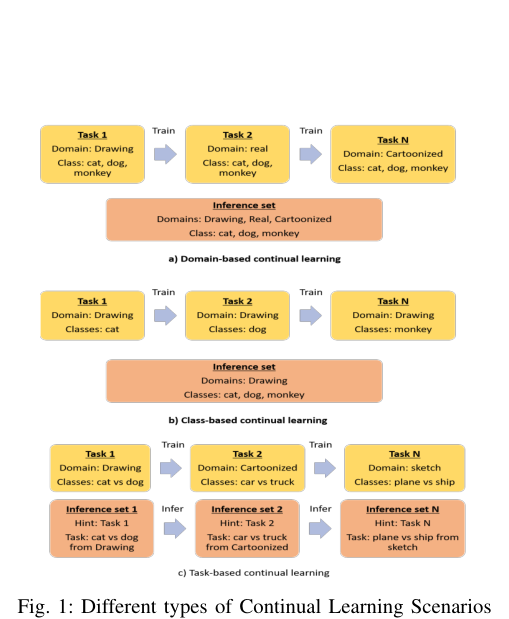
\includegraphics[width=0.75\textwidth,height=0.4\textheight,keepaspectratio]{figures/2512.16871_p2.png}\end{center}

The figure displays three flowcharts (a, b, and c) representing different continual learning scenarios, each consisting of a sequence of yellow task boxes connected by gray arrows labeled "Train." Each task box specifies a domain and a set of classes, followed by a larger orange "Inference set" box that lists the cumulative domains and classes encountered. The diagrams distinguish between domain-based learning (changing domains with same classes), class-based learning (same domain with changing classes), and task-based learning (changing both domains and classes).

**Reducing Catastrophic Forgetting in Online Class Incremental Learning
  Using Self-Distillation** — \citep{2409.11329} p.4

\begin{center}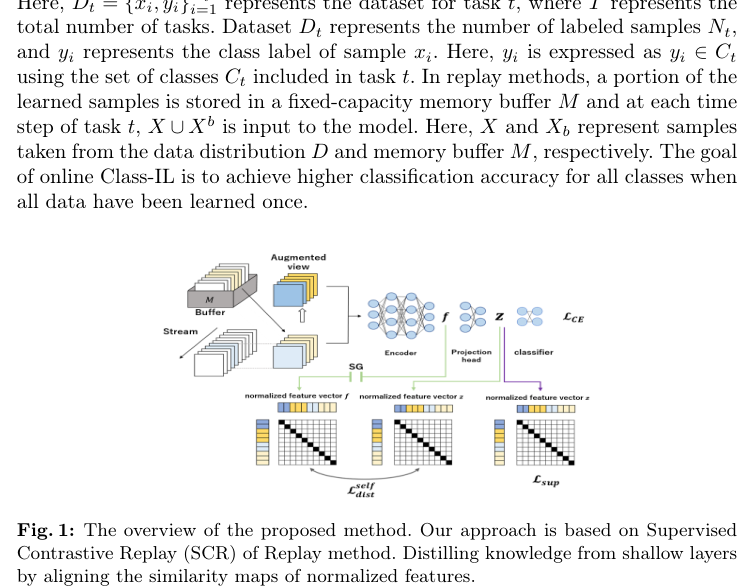
\includegraphics[width=0.75\textwidth,height=0.4\textheight,keepaspectratio]{figures/2409.11329_p4.png}\end{center}

The figure illustrates a workflow where a data stream and a memory buffer are processed through an encoder, a projection head, and a classifier to compute various losses, including \$L\_\{CE\}\$. Below the main architecture, three similarity matrices represent normalized feature vectors \$\textbackslash{}mathbf\{f\}\$, \$\textbackslash{}mathbf\{x\}\$, and \$\textbackslash{}mathbf\{z\}\$, which are used to calculate self-distillation loss (\$L\_\{self\textbackslash{}\_dist\}\$) and supervised loss (\$L\_\{sup\}\$) by aligning similarity maps. The diagram conveys a supervised contrastive replay method that uses feature similarity alignment to mitigate catastrophic forgetting.

**Mitigating Catastrophic Forgetting in Task-Incremental Continual
  Learning with Adaptive Classification Criterion** — \citep{2305.12270} p.1

\begin{center}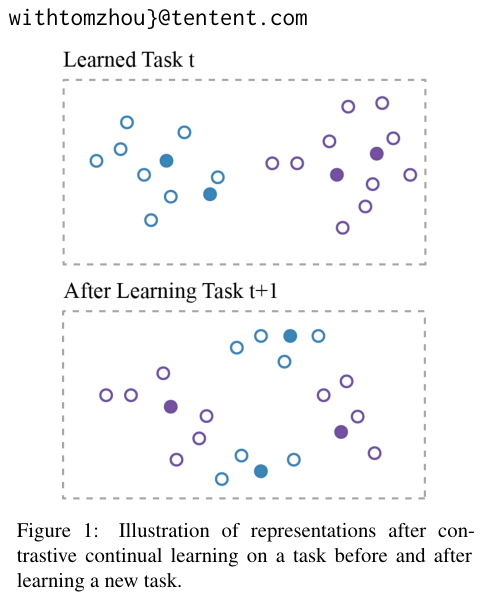
\includegraphics[width=0.75\textwidth,height=0.4\textheight,keepaspectratio]{figures/2305.12270_p1.png}\end{center}

The figure consists of two dashed rectangular boxes containing sets of colored circles (blue and purple) representing data representations. The top box, labeled "Learned Task t," shows the blue and purple circles clearly separated into two distinct clusters, while the bottom box, labeled "After Learning Task t+1," shows the blue and purple circles intermingled, conveying how learning a new task can cause representations of previous tasks to overlap.

**Efficient Rehearsal Free Zero Forgetting Continual Learning using
  Adaptive Weight Modulation** — \citep{2311.15276} p.5

\begin{center}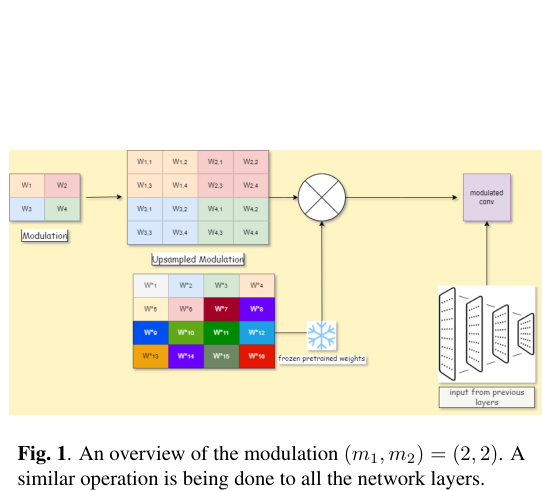
\includegraphics[width=0.75\textwidth,height=0.4\textheight,keepaspectratio]{figures/2311.15276_p5.png}\end{center}

The figure illustrates the modulation process where a \$2 \textbackslash{}times 2\$ modulation matrix is upsampled to match the dimensions of a \$4 \textbackslash{}times 4\$ pretrained weight matrix. An element-wise multiplication operation is performed between the upsampled modulation and the frozen pretrained weights to produce a modulated convolutional layer.

\textbf{STAR: Stability-Inducing Weight Perturbation for Continual Learning} — \citep{2503.01595} p.2

\begin{center}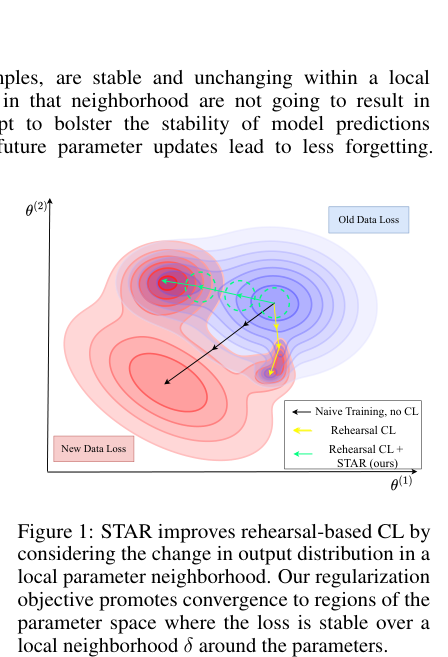
\includegraphics[width=0.75\textwidth,height=0.4\textheight,keepaspectratio]{figures/2503.01595_p2.png}\end{center}

The figure displays a 2D contour plot representing loss landscapes for "Old Data Loss" and "New Data Loss" across parameter axes \$\textbackslash{}theta\textasciicircum{}\{(1)\}\$ and \$\textbackslash{}theta\textasciicircum{}\{(2)\}\$. Arrows indicate different training trajectories: a black arrow shows "Naive Training, no CL" moving toward the new data loss, a yellow arrow shows "Rehearsal CL" moving toward the old data loss, and a cyan arrow shows "Rehearsal CL + STAR (ours)" moving toward a stable region where both loss contours overlap.

\textbf{Learning to Continually Learn with the Bayesian Principle} — \citep{2405.18758} p.3

\begin{center}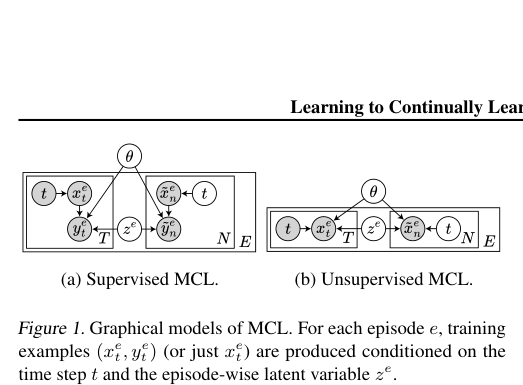
\includegraphics[width=0.75\textwidth,height=0.4\textheight,keepaspectratio]{figures/2405.18758_p3.png}\end{center}

The figure presents two directed acyclic graphs representing the graphical models for Supervised MCL (a) and Unsupervised MCL (b). In both models, a parameter node \$\textbackslash{}theta\$ points to latent variables, while nodes representing data (such as \$x\_t\textasciicircum{}e\$, \$y\_t\textasciicircum{}e\$, and \$z\textasciicircum{}e\$) are connected by arrows to indicate probabilistic dependencies across time steps \$t\$ and episodes \$e\$.

\textbf{Saliency-Augmented Memory Completion for Continual Learning} — \citep{2212.13242} p.3

\begin{center}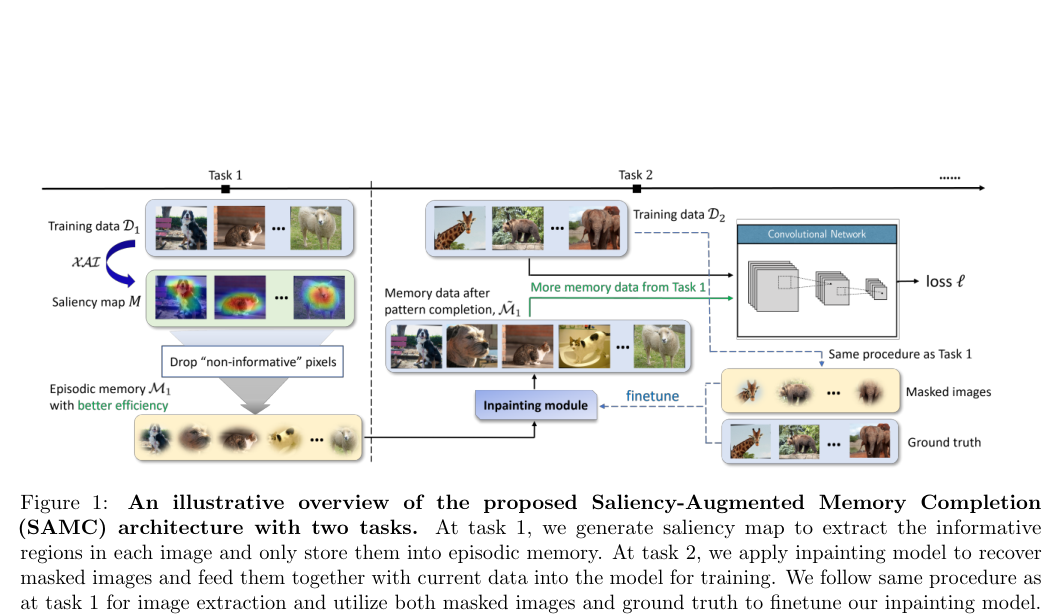
\includegraphics[width=0.75\textwidth,height=0.4\textheight,keepaspectratio]{figures/2212.13242_p3.png}\end{center}

The figure illustrates the SAMC architecture across two tasks, using arrows to show the flow from training data \$\textbackslash{}mathcal\{D\}\_1\$ through an XAI process that generates saliency maps \$\textbackslash{}mathcal\{M\}\$ to extract informative pixels for episodic memory \$\textbackslash{}mathcal\{M\}\_1\$. During Task 2, the diagram shows the inpainting module recovering masked images from \$\textbackslash{}mathcal\{M\}\_1\$ to be used alongside training data \$\textbackslash{}mathcal\{D\}\_2\$ for training a convolutional network, while simultaneously using masked images and ground truth to finetune the inpainting module.

\textbf{Forward-Only Continual Learning} — \citep{2509.01533} p.3

\begin{center}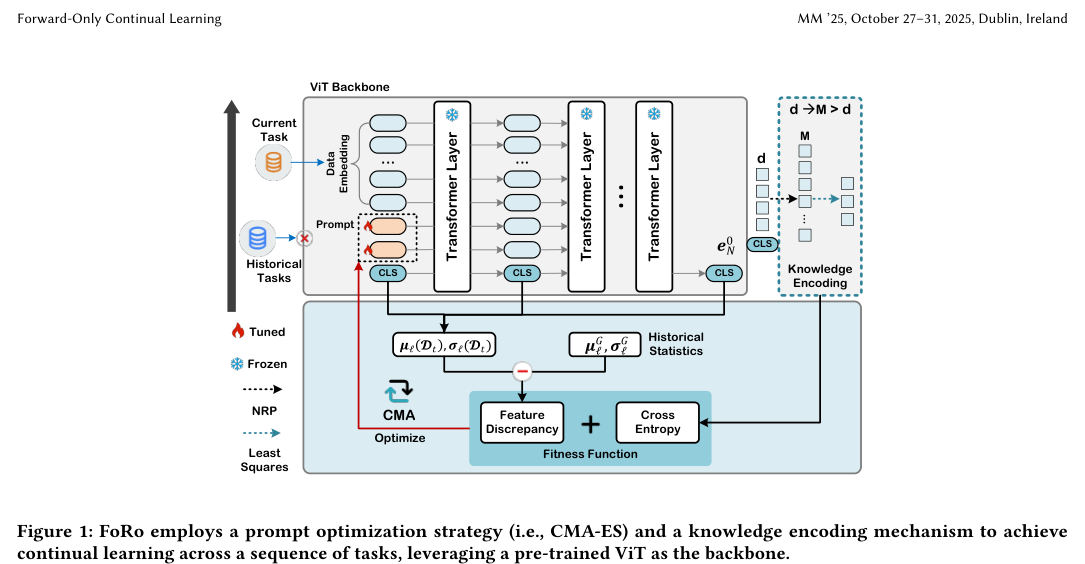
\includegraphics[width=0.75\textwidth,height=0.4\textheight,keepaspectratio]{figures/2509.01533_p3.png}\end{center}

The figure illustrates the FoRo architecture, which utilizes a pre-trained ViT backbone composed of frozen transformer layers and tunable prompt embeddings. It depicts a training loop where a CMA-ES optimization strategy minimizes a fitness function—comprising feature discrepancy and cross-entropy—based on historical statistics (\$\textbackslash{}mu\_t\textasciicircum{}H, \textbackslash{}sigma\_t\textasciicircum{}H\$) and current task data. A knowledge encoding mechanism is shown mapping the output of the final transformer layer to a dimension \$d \textbackslash{}to M > d\$ to facilitate continual learning.

**Efficient Meta-Learning for Continual Learning with Taylor Expansion
  Approximation** — \citep{2210.00713} p.6

\begin{center}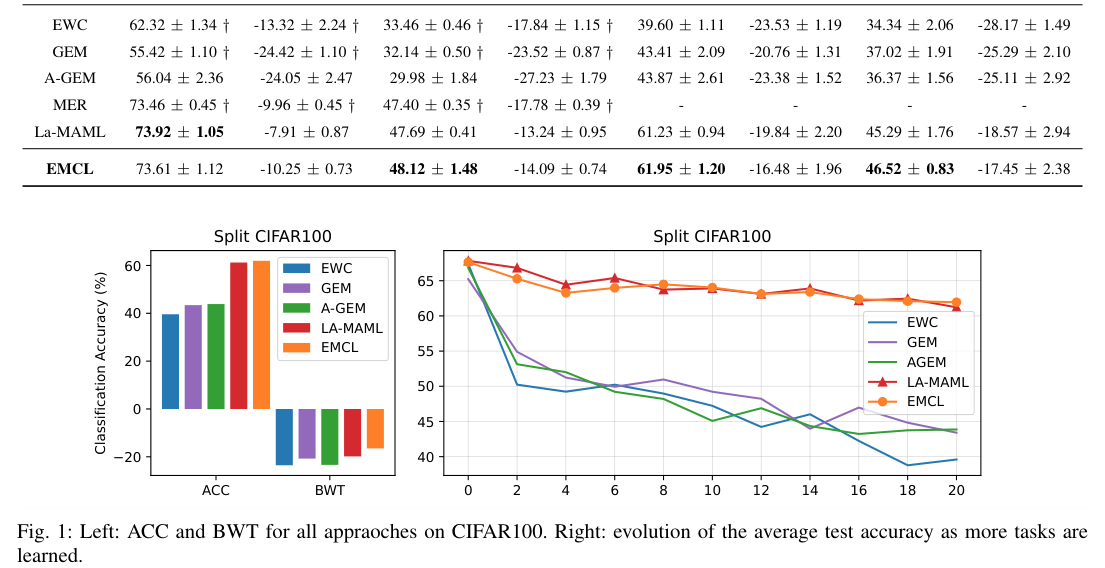
\includegraphics[width=0.75\textwidth,height=0.4\textheight,keepaspectratio]{figures/2210.00713_p6.png}\end{center}

The figure consists of a table of performance metrics and two bar/line charts comparing different continual learning methods on the Split CIFAR100 dataset. The left bar chart compares the Accuracy (ACC) and Backward Transfer (BWT) for EWC, GEM, A-GEM, La-MAML, and EMCL, while the right line chart plots the evolution of average test accuracy across 20 tasks for each method. Overall, the figure conveys that EMCL achieves competitive accuracy and improved backward transfer compared to the baseline methods.

\textbf{Predicting the Susceptibility of Examples to Catastrophic Forgetting} — \citep{2406.09935} p.2

\begin{center}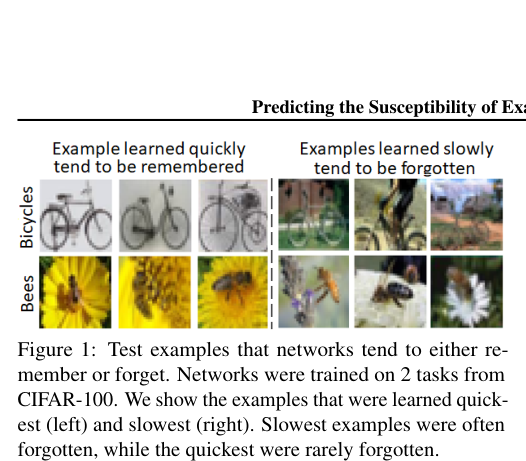
\includegraphics[width=0.75\textwidth,height=0.4\textheight,keepaspectratio]{figures/2406.09935_p2.png}\end{center}

The figure displays a grid of image samples from the CIFAR-100 dataset, organized into two main columns labeled "Example learned quickly tend to be remembered" and "Examples learned slowly tend to be forgotten." The rows categorize these images into two classes: "Bicycles" and "Bees." The figure conveys that examples learned rapidly by the network are more likely to be retained, whereas those learned slowly are more susceptible to being forgotten.

\textbf{Slowing Down Forgetting in Continual Learning} — \citep{2411.06916} p.4

\begin{center}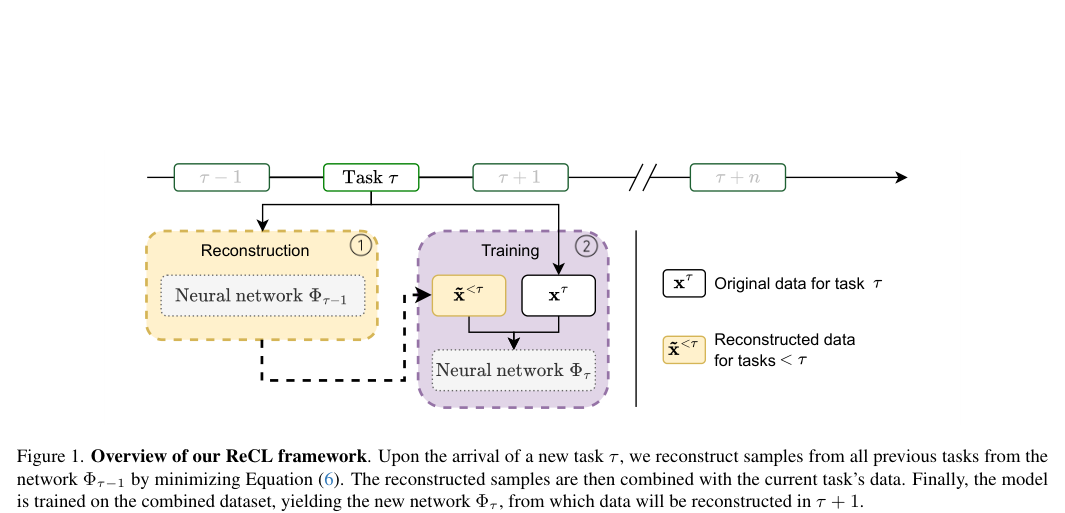
\includegraphics[width=0.75\textwidth,height=0.4\textheight,keepaspectratio]{figures/2411.06916_p4.png}\end{center}

The figure illustrates the ReCL framework through a timeline of tasks (\$\textbackslash{}tau-1\$ to \$\textbackslash{}tau+n\$) and a two-step process for task \$\textbackslash{}tau\$. Step 1 shows a "Reconstruction" block where the previous neural network \$\textbackslash{}Phi\_\{\textbackslash{}tau-1\}\$ generates reconstructed data \$\textbackslash{}tilde\{\textbackslash{}mathbf\{x\}\}\textasciicircum{}\{<\textbackslash{}tau\}\$, which is then combined with the original data \$\textbackslash{}mathbf\{x\}\textasciicircum{}\textbackslash{}tau\$ in Step 2 for "Training" the new neural network \$\textbackslash{}Phi\_\textbackslash{}tau\$.

\textbf{Learning to Continually Learn} — \citep{2002.09571} p.3

\begin{center}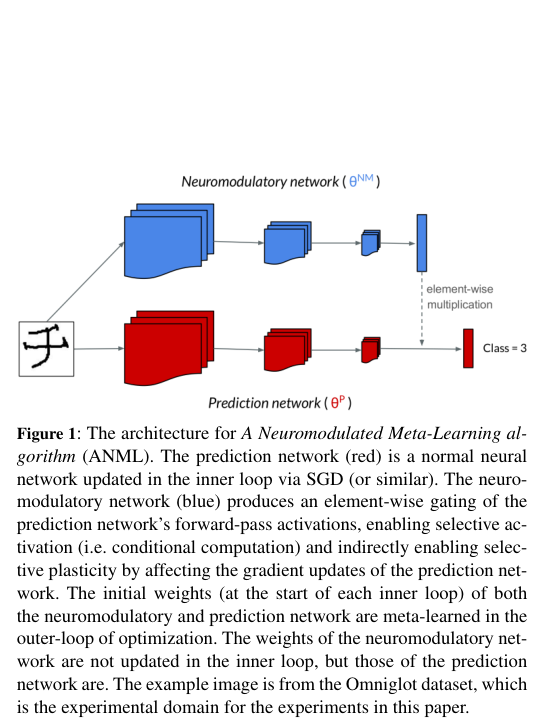
\includegraphics[width=0.75\textwidth,height=0.4\textheight,keepaspectratio]{figures/2002.09571_p3.png}\end{center}

The figure illustrates the architecture of the A Neuromodulated Meta-Learning (ANML) algorithm, showing a sample image from the Omniglot dataset being processed through two parallel paths. A blue neuromodulatory network (\$\textbackslash{}theta\textasciicircum{}\{NM\}\$) produces activations that undergo element-wise multiplication with the activations of a red prediction network (\$\textbackslash{}theta\textasciicircum{}P\$) to gate the prediction network's forward pass. This mechanism enables selective activation and indirectly enables selective plasticity by affecting the prediction network's gradient updates.


\bibliographystyle{unsrtnat}
\bibliography{refs}

\end{document}
